%----------------------------------------------------------------------------
\chapter{\bevezetes}
%----------------------------------------------------------------------------

%----------------------------------------------------------------------------
\section{Problem Definition}
%----------------------------------------------------------------------------

One of the most popular trend in the IT industry today is the cloud and the migration of enterprise workloads from private data centers into public cloud solutions. This direction is not surprising, as cloud computing offers a lot of benefits for companies, like minimizing operational costs, flexibility, ease of use -- just to mention a few \cite{CloudComputingStatistics}. The growing pace of enterprise cloud adoption causes that more and more applications move into the reigns of public cloud providers. It is not uncommon that these cloud based applications support some fundamental aspects of everyday life like online banking, telecommunications, healthcare, so they can be viewed -- without exaggeration -- critical systems that require a certain level of reliability from the underlying infrastructure.

Kubernetes became the number one choice for managing cloud based systems as it provides a vastly configurable, modular way of deploying and operating distributed, container based applications. However, the high abstraction layer that Kubernetes brings into the creation and the maintenance of applications causes some earlier well defined concepts, such as dependability harder to guarantee and reason about.

%\begin{itemize}
%	\item enterprise cloud adoption is growing fast (https://findstack.com/cloud-computing-statistics/)
%	\item lot of critical applications move to the cloud (banking, telco, datastores, software companies, tools) (TODO source)
%	\item many of the cloud base applications can be viewed as critical systems (lot of money at stake, communication at stake - implicitly can cause human harm, \etc)
%	\item \etc
%\end{itemize}

%----------------------------------------------------------------------------
\section{Motivation}
%----------------------------------------------------------------------------

Applications running in the cloud are inherently exposed to a quite dynamic environment. The infrastructure layer under the application can frequently change causing different kind of anomalies and failures on the application level. In most cases, the physical hardware on which the software of a cloud tenant -- a company or individual customer, who uses a set of services at a cloud provider -- runs is not accessible for the users. This means that the implementation of fault tolerant and justifiably reliable applications must be handled on higher abstraction layers that are available for cloud users.

As the number of cloud based mission critical systems constantly rise, it is indispensable to provide various techniques to be able guarantee a given level of dependability of these applications. The Kubernetes ecosystem supports many building blocks to achieve this goal, however, arranging and integrating these units to form a practically usable and efficient structure can be a daunting task.

%\begin{itemize}
%	\item dependability of cloud based applications should be constantly monitored and guaranteed
%	\item achieving highly reliable and robust cloud applications
%	\item prepare the cloud application for various kind of failures, anomalies
%	\item \etc
%\end{itemize}

%----------------------------------------------------------------------------
\section{Goals}
%----------------------------------------------------------------------------

The goals of this thesis work include the below described notions.

First, introducing Kubernetes -- a widely used system for automating deployment, scaling, and management of containerized applications in the cloud -- is needed to collect the necessary knowledge in order to be able understand the rest of the work.

Following that, the procedure of measuring dependability in a distributed, Kubernetes based system will be defined, which includes reinterpreting and adopting the concept of dependability tailored for this environment.

The newly constructed methods to determine the dependability will be demonstrated with the help of a custom made sample application to serve as a case study on the Kubernetes platform.

After the sample application and the collection of dependability metrics are functional, the possible alternatives to improve the dependability of the app are investigated in different layers of the Kubernetes based deployment. The goals include the implementation and detailed description of some of these enhancements.

In order to be able to measure the effects of the implemented enhancements, a test framework is needed. The framework shall support fault injection mechanisms to allow assessing the dependability of the application in various kinds of scenarios.

Lastly, the measurement results should be presented and evaluated, summarizing the gained experiences.

The visualized overview of the thesis' objectives can be seen in Figure \ref{fig:overview}.


%\begin{itemize}
%	\item introduce Kubernetes a widely used system for automating deployment, scaling, and management of containerized applications in the cloud
%	\item define a way to measure dependability metrics in Kubernetes based environments
%	\item create a sample application on the Kubernetes platform to demonstrate the collection of dependability metrics
%	\item investigate the possible alternatives to improve the dependability in different layers of the Kubernetes based deployment/application and implement some of them
%	\item create a framework with fault injection capabilities to measure the effects of the above mentioned improvements
%	\item present and evaluate the measurement results and summarize the gained experiences
%\end{itemize}

\begin{figure}[H]
	\centering
	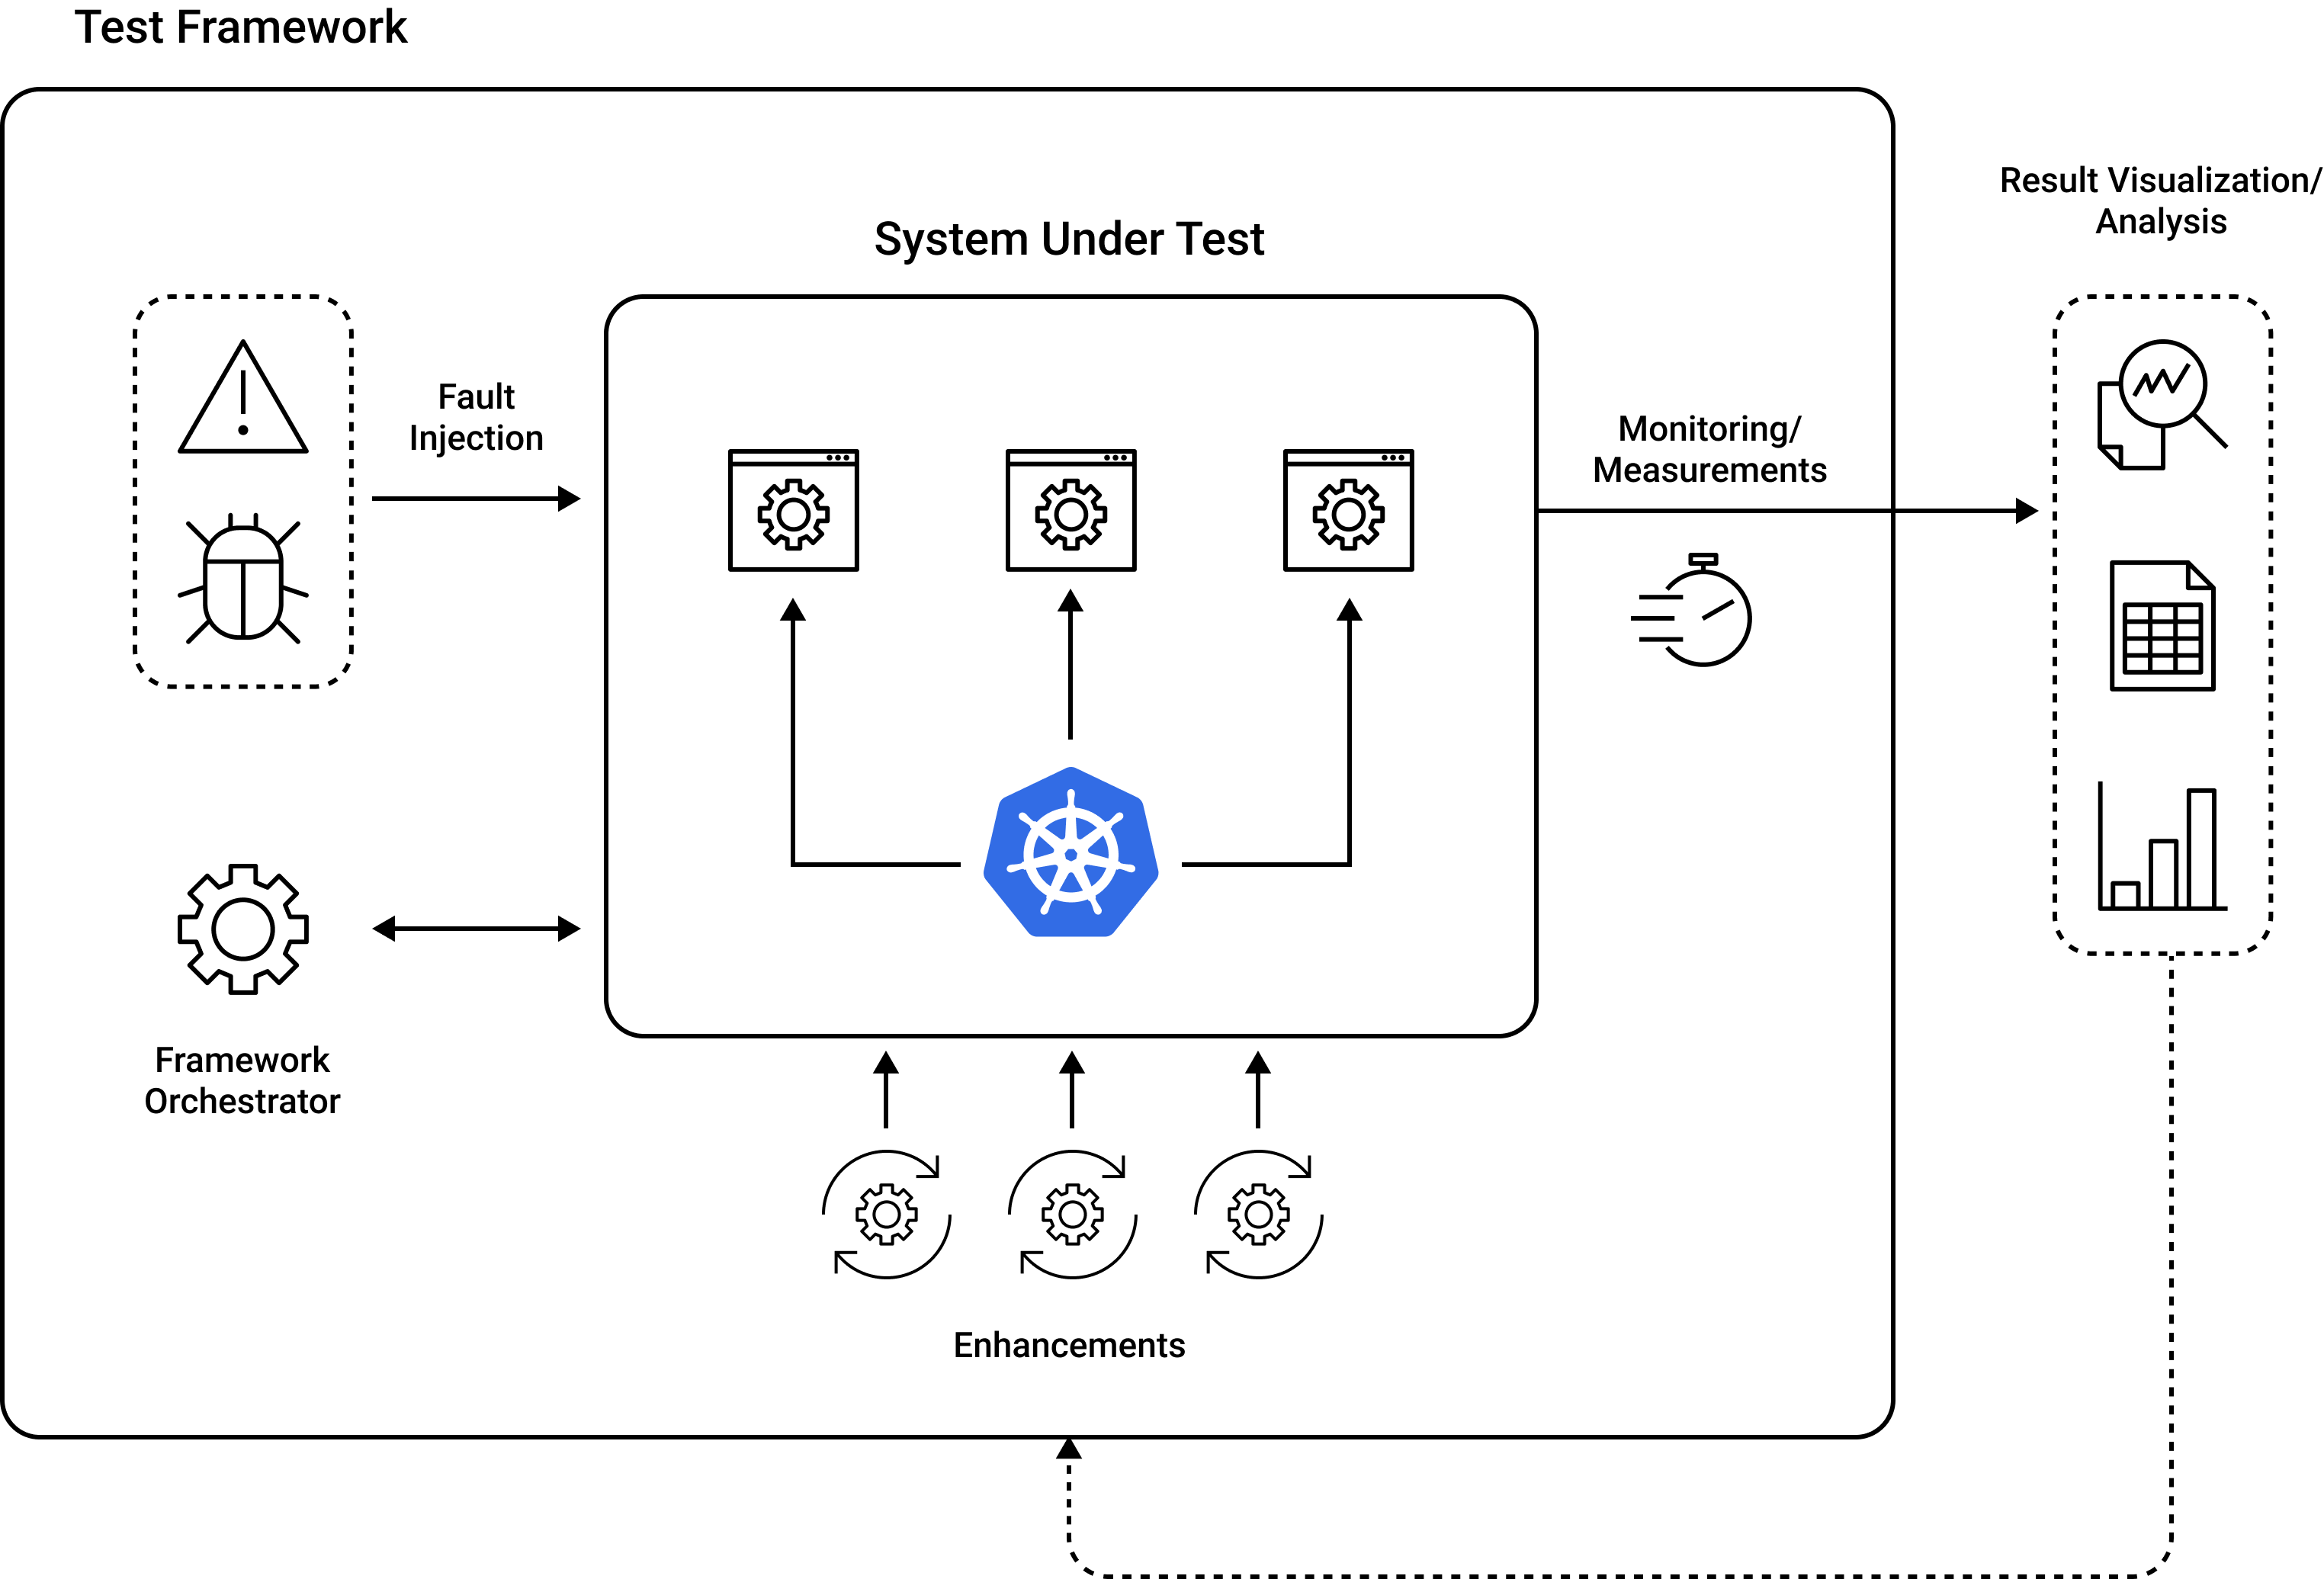
\includegraphics[width=140mm, keepaspectratio]{figures/overview-diagram.png}
	\caption{Overview diagram}
	\label{fig:overview}
\end{figure}

%----------------------------------------------------------------------------
\section{Thesis structure}
%----------------------------------------------------------------------------

The thesis documentation is structured in a way to attempt allowing straightforward comprehension. The thesis first gives a brief overview about the background knowledge used throughout the project, listing and describing the technologies and concepts applied during the work (see Chapter \ref{background}). This chapter is followed by the detailed presenting of the sample application that is will be used to demonstrate the features of the test framework (see Chapter \ref{sample-app}). The test framework is introduced in the Chapter \ref{test-framework} including both the related aspects of design and implementation. Then, the possible alternatives for improving dependability and two implementations are described in Chapter \ref{enhancements} which are later evaluated in Chapter \ref{evaluation}. Finally, some potential future developments and related works are discussed in Chapter \ref{future-work} and in Chapter \ref{related-works}.

%\begin{itemize}
%	\item to make the results and the thinking easier to comprehend, the thesis in the following way
%	\item background
%	\item sample application - design and implementation - this will be used the demonstrate the features of the test framework
%	\item test framework
%	\item enhancements - alternatives to improve the dependability of the sample application
%\end{itemize}

























